\subsection{Simulation}

The behaviour of the impementation was tested by writing small programs that would try to provoke certain errors and write debug data to the registers. They were then simulated, and the resulting data in the registers was compared to the desired data.

Alu operations, memory operations, forwarding, jumping, branching and flushing were all tested and proved to work correctly.


\todo{Insert programs into appendix?}

\subsection{Timing Simulation}

\begin{figure}[ht]
    \centering
    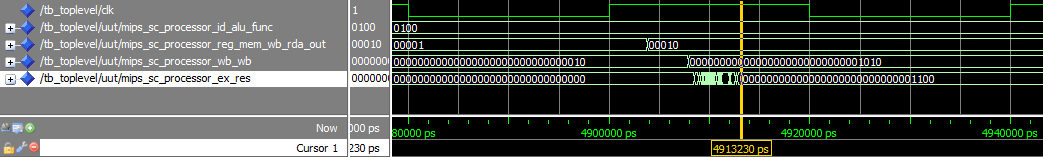
\includegraphics[scale=0.5]{figures/TimingSimulation.png}
    \caption{Timing diagram for critical path} 
    \label{fig:timing}
\end{figure}

Figure \ref{fig:timing} is a timing diagram showing the output from the ALU, which is the end of the critical path that starts at the ex/mem pipeline register and goes through the bottom link mux, the forwarding unit, the forwarding mux, and into the ALU.
The time from a rising clock edge to a the output is stable is shown to be $13.230$ ns, which translates to a maximum clock speed of about $75$ Mhz.
This is very close to the max clock speed of $77.442$ MHz reported by the synthesis tool.

\subsection{Verification}

By following the procedure in the compendium \cite[p.47]{lab-compendium}, the design was added to the Micro Blaze framework

\begin{figure}[ht]
    \centering
    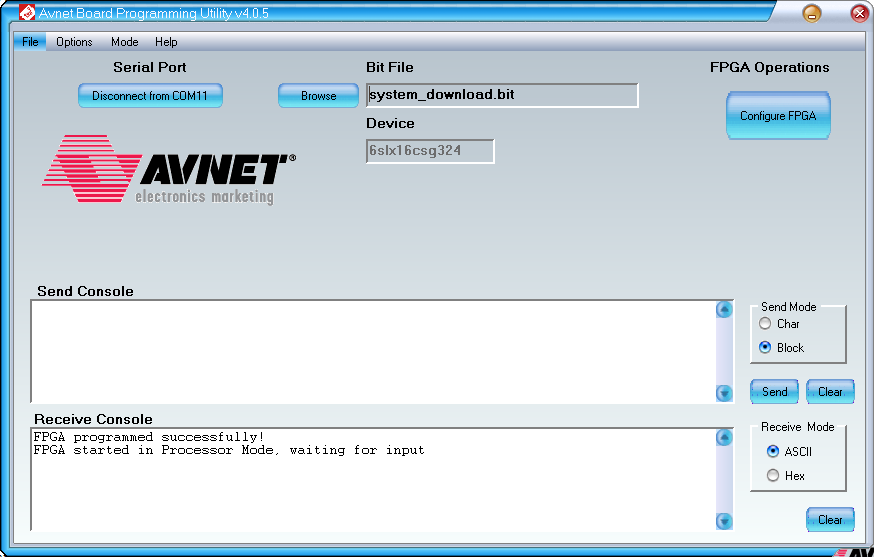
\includegraphics[scale=0.5]{figures/AVNET.png}
    \caption{FPGA programmed successfully} 
    \label{fig:avprog}
\end{figure}

\todo{stuff}

